\documentclass[a4paper]{article}
\usepackage[document]{ragged2e}
%\usepackage{simplemargins}

%\usepackage[square]{natbib}
\usepackage{mathtools}
\usepackage{amsfonts}
\usepackage{amssymb}
\usepackage{graphicx}
\usepackage{tabularx}
\usepackage[export]{adjustbox}
\usepackage[numbered,framed]{matlab-prettifier}
\usepackage{minted}
\usepackage{svg}
\usepackage{graphicx}
\usepackage{fancyhdr}
\pagestyle{fancy}
\usepackage{xcolor}
\usepackage{lipsum}
\setlength\headheight{26pt} %% just to make warning go away. Adjust the value after looking into the warning.
\lfoot{{\small\textsf{\thepage}}}
\rfoot{\small\textsf{\today}}
\cfoot{}
\rhead{
\includegraphics[width=50pt]{bigcat}}
\lhead{
\includegraphics[width=30pt]{ssn}}
\begin{document}
% \pagenumbering{gobble}

\Large
 \begin{center}
BigCat Wireless - EC401\\
\textbf{Assignment 5}

\hspace{10pt}

% Author names and affiliations
\large
Vignesh Mohan\\
\smallskip
\small
183002181\\
\small
Electronics and Communication Department\\
\small
Sri Sivasubramiya Nadar College of Engineering, 603110\\
\end{center}

\hspace{10pt}
\normalsize

\textit{1. Describe why OFDMA is not being used in both uplink and downlink.}\\
\begin{itemize}
    \item Signals that demand linear amplification and have a high Peak-to-Average Power Ratio (PAPR) do not lend itself to the usage of efficient RF power amplifiers. As a result, it is important to choose a transmission mode that operates at a nearly constant power level.
    
    \item But OFDMA has a very high PAPR, and the power amplifier required for such large ranges cannot be constructed in User Equipment (UE) as it is necessary to ensure that the UE use as little battery power as possible. Hence, SC-FDMA is used for uplink, as it has a lower PAPR.
    s
    \item Base Stations (BS), on the other hand, use OFDMA for downlink because they have more than enough resources to handle high PAPR.
\end{itemize}

\bigskip

\textit{2. List the Challenges/Disadvantages of SC-FDMA.}\\
\begin{itemize}
  \item SC-FDMA has higher inter symbol interference (ISI).
  \item SC-FDMA generally provides a less flexible resource allocation and lesser spectral efficiency compared to OFDMA,
  \item Multipath fading affects SC-FDMA, but OFDMA is more resilient to it.
  \item In comparison to OFDM, Channel estimation with pilots is more difficult in SC-FDMA because you don't have orthogonal data on each frequency bin.
\end{itemize}

\bigskip
\textit{3. Create a Matlab Model as following:\\[10pt]
    • Bandwidth: 20MHz, Fs: 30.72, FFT size: 2048 \\
    • Generate bit stream and Map to 16-QAM (Modulation symbol length <= 1200) 
            i. u(1:1200) \\
    • Apply DFT spread (SC-FDMA)\\
    • Map the Modulation symbols(1200) to IFFT input (2048) as shown below\\
    • Apply IFFT \\
    • Calculate PAPR (with DFT spread and without DFT spread) \\
    • Create Spectrum plot for both cases\\
}
\bigskip
\definecolor{bg}{rgb}{0.95,0.95,0.95}
\begin{minted}[linenos=true,bgcolor=bg]{matlab}
% ofdma_scfdma.m
bw = 20; % (in MHz)
Fs = 30.72; % (in Hz)
fftSize = 2048;
num_data_samples = 4800;
M = 16; % Modulation order
k = log2(M); % bits per sym

inputData = randi([0 1], num_data_samples, 1);
%reshape into k bit matrix and then convert to decimal values
inputDataMat = reshape(inputData, length(inputData)/k, k);
inputSym = bi2de(inputDataMat);
modData = qammod(inputSym, M); % M-QAM modulation
% Serial to Parallel data
dataParallel = reshape(modData, 1200, []);
scfdmaData = fft(dataParallel, 1200, 1); % apply DFT spread

% map the Modulation symbols(1200) to IFFT input (2048)
ifftOFDM = [(0); modData(1:600); zeros(847, 1);...
    modData(601:1200)];
ifftSCFDMA = [[0]; scfdmaData(1:600); zeros(847, 1); ...
    scfdmaData(601:1200)];

% Apply IFFT
dataSCFDMA = ifft(ifftSCFDMA, fftSize, 1);
dataOFDM = ifft(ifftOFDM, fftSize, 1);

% PAPR
paprSCFDMA = max((abs(dataSCFDMA)).^2)/...
    mean((abs(dataSCFDMA)).^2);
paprOFDM = max((abs(dataOFDM)).^2)/..
    mean((abs(dataOFDM)).^2);

fprintf("PAPR (SC-FDMA) = %.6f\n", paprSCFDMA);
fprintf("PAPR (OFDM) = %.6f\n", paprOFDM);
\end{minted}
Output:\\[10pt]
PAPR (SC-FDMA) = 5.734021\\
PAPR (OFDM) = 7.587032\\
\begin{figure}[hbt!]
    \centering
  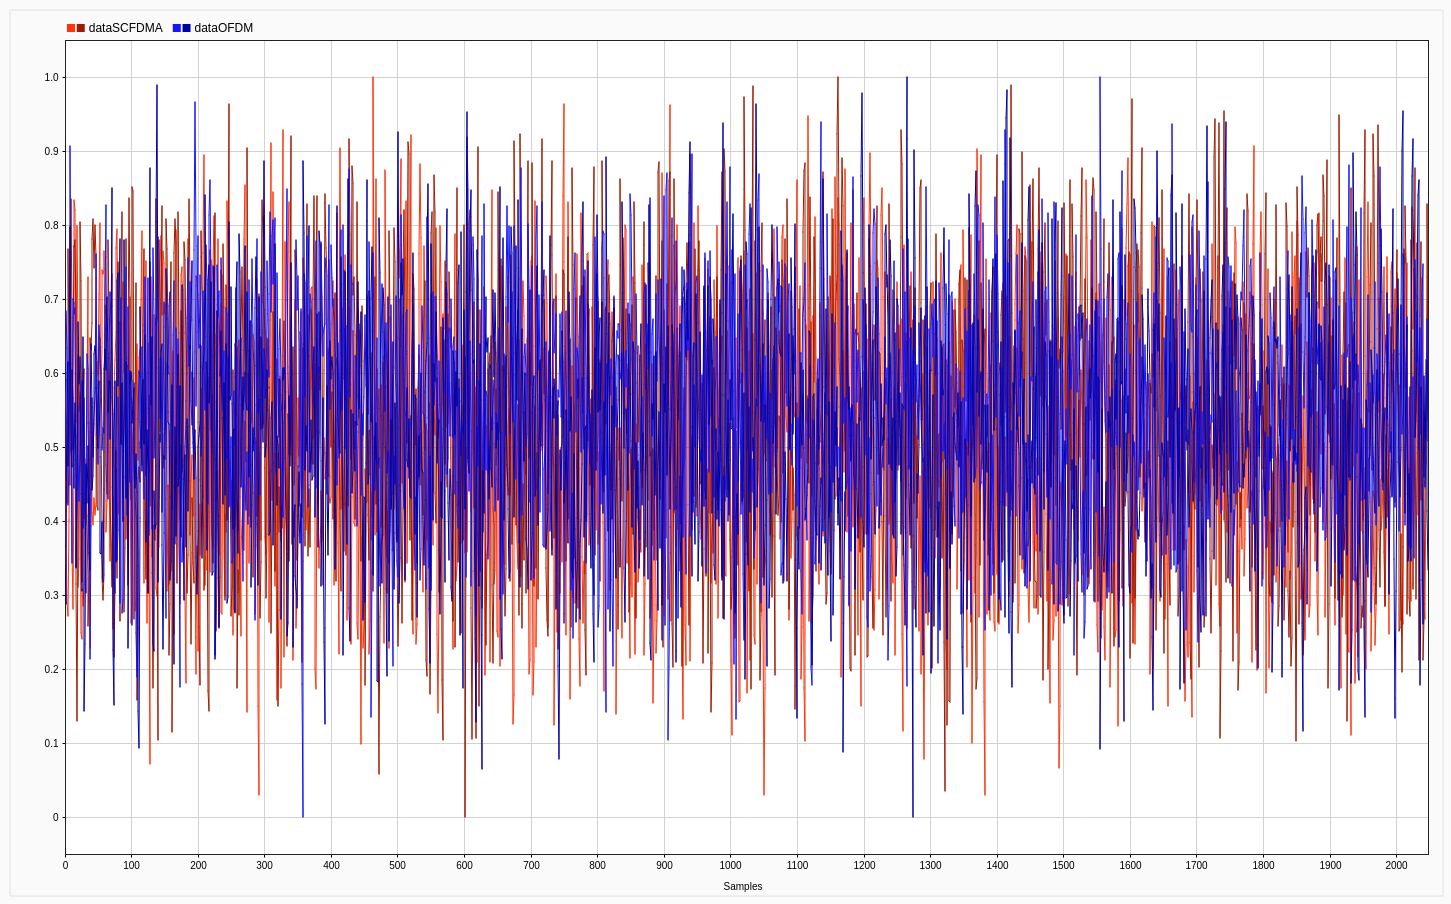
\includegraphics[width=\linewidth]{ofdm_scfdma_data}
  \caption{Plot of OFDM and SC-FDMA data signals (normalized)}
\end{figure}
\begin{figure}[hbt!]
    \centering
  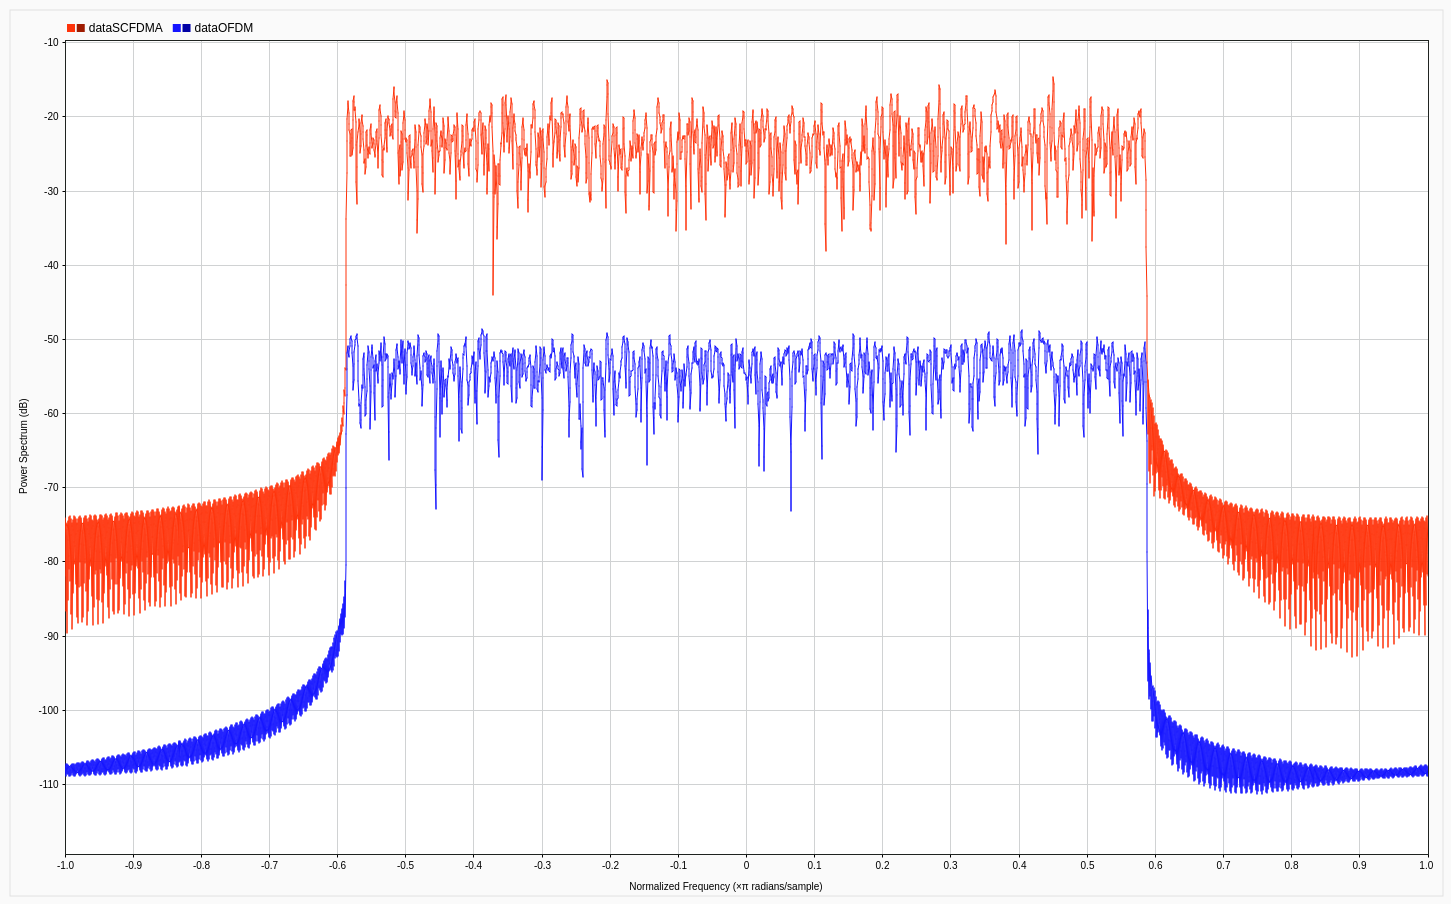
\includegraphics[width=\linewidth]{ofdm_scfdma_spectrum}
  \caption{Power Spectrum of OFDM and SC-FDMA signals}
\end{figure}
\end{document}